\begin{figure}
    \centering
    \begin{subfigure}[b]{0.49\linewidth}
    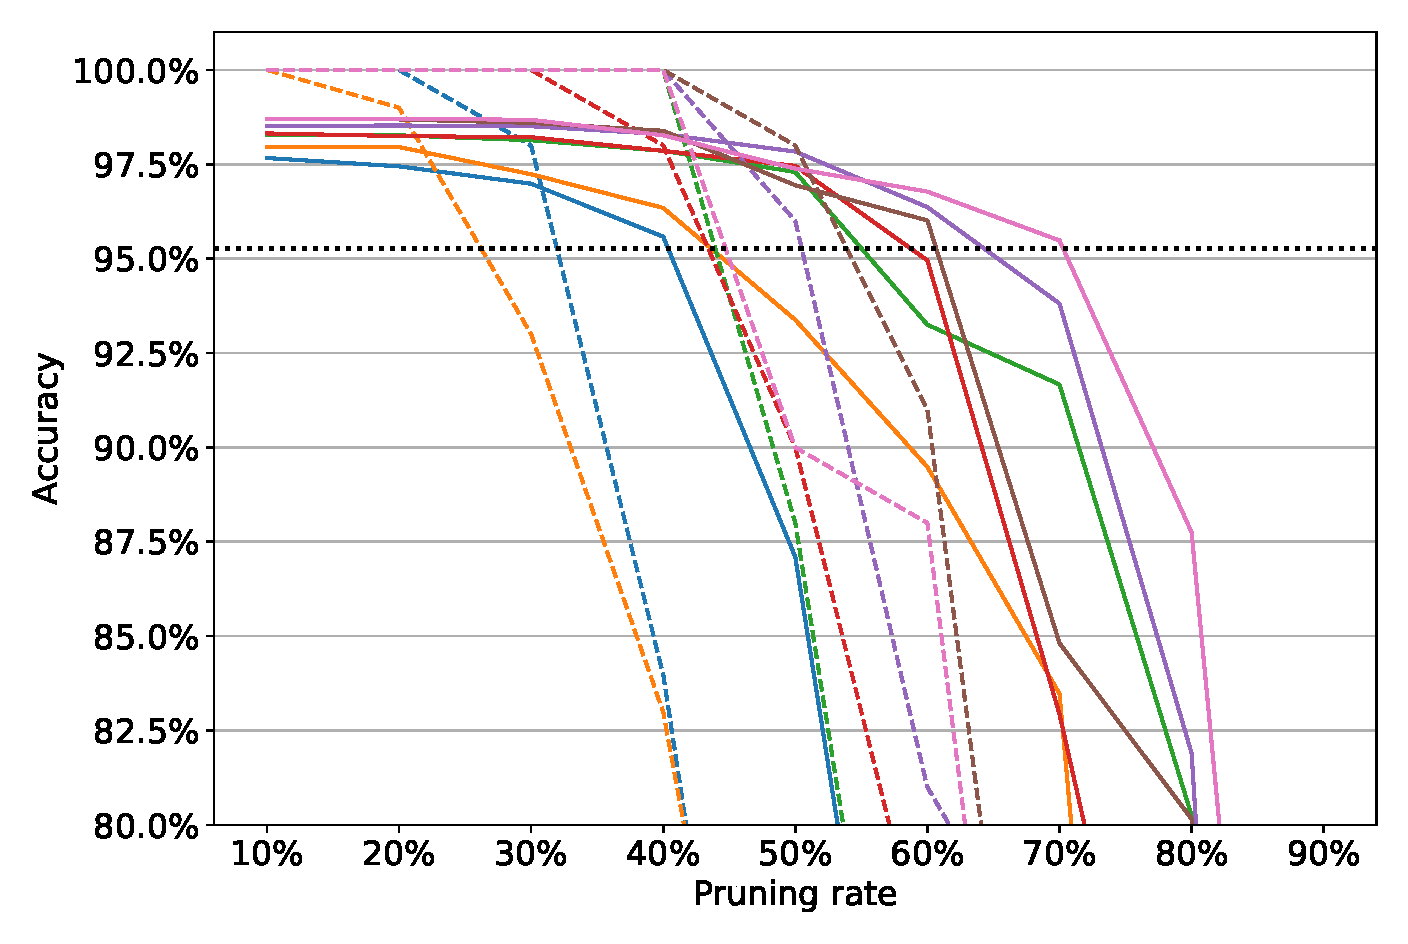
\includegraphics[width = \linewidth]{images/frontier/frontier_influence_epsilon_pruning_lenet1.eps}
    \caption{LeNet-1}
    \label{fig:frontier_influence_epsilon_pruning-a}
    \end{subfigure}
    \begin{subfigure}[b]{0.49\linewidth}
    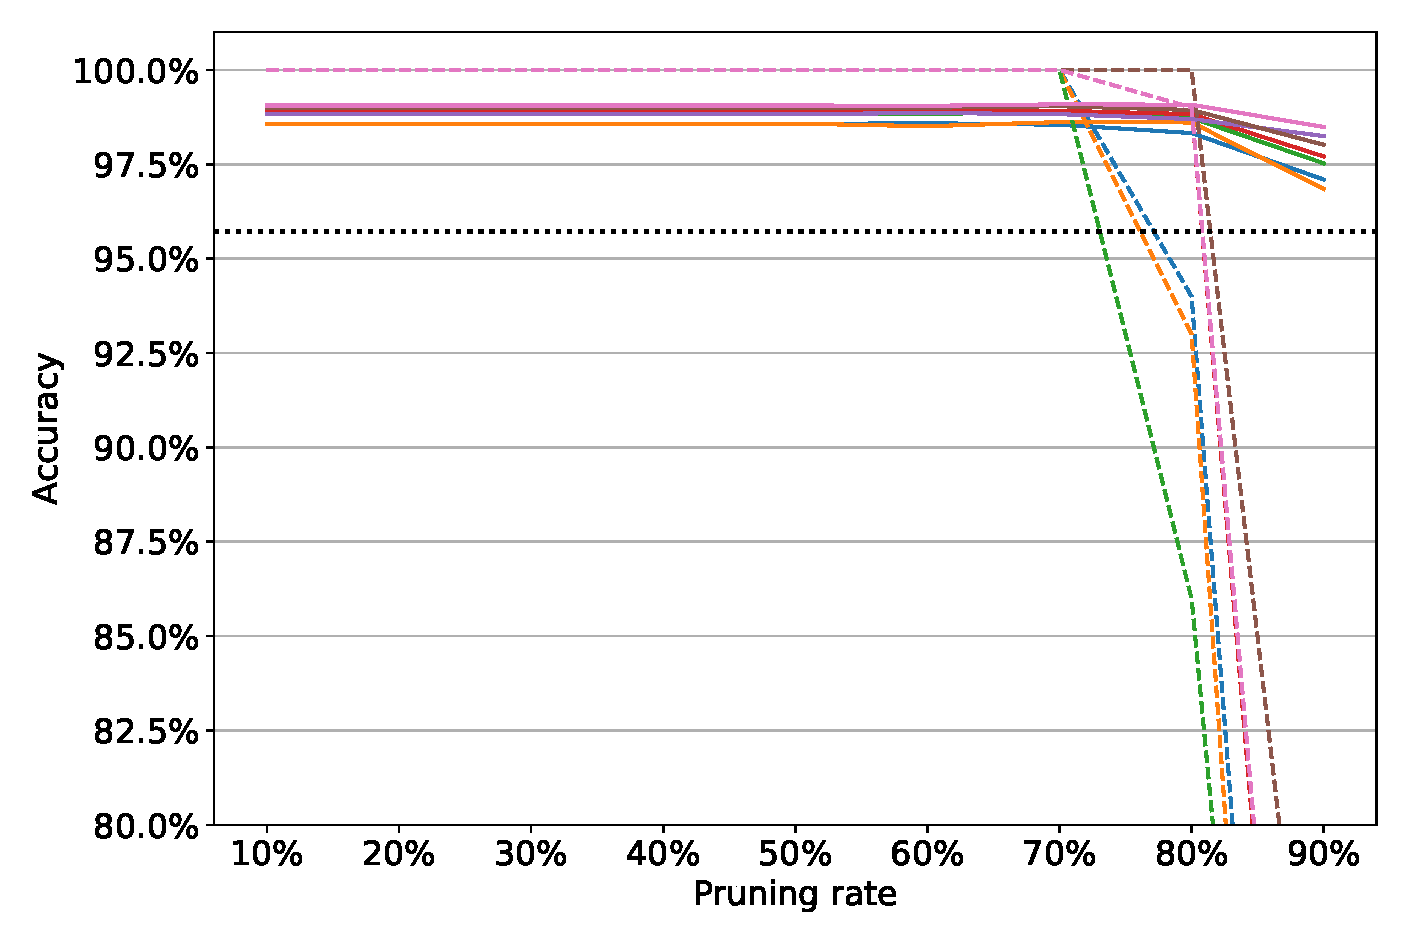
\includegraphics[width = \linewidth]{images/frontier/frontier_influence_epsilon_pruning_lenet5.eps}
    \caption{LeNet-5}
    \label{fig:frontier_influence_epsilon_pruning-b}
    \end{subfigure}
    \begin{subfigure}[b]{\linewidth}
    \centering
    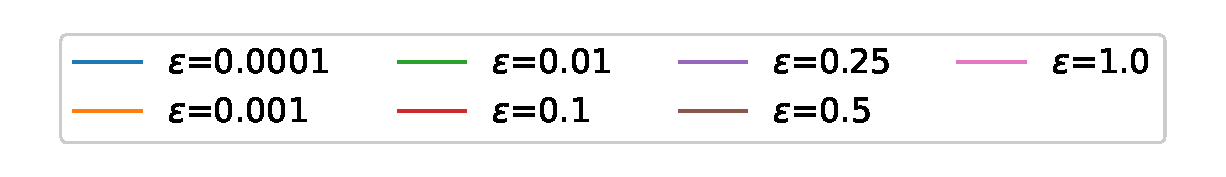
\includegraphics[height=1cm]{images/frontier/legend_frontier_pruning_perarch_colors.eps}
    \quad
    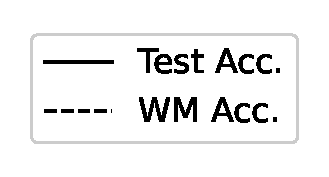
\includegraphics[height=1cm]{images/frontier/legend_frontier_pruning_perarch_linetypes.eps}
    \end{subfigure}
    
    \caption{Model accuracy after pruning attacks with pruning rates from 10\% to 90\%. The black dotted line indicates the threshold for the maximal plausible pruning attack.}
    \label{fig:frontier_influence_epsilon_pruning}
\end{figure}